Comparado a las estructuras de datos lineales como las listas enlazadas y arreglos unidimensionales, que tienen un método canónico de recorrido, las estructuras arborescentes pueden ser recorridas de muchas maneras diferentes. Comenzando en la raíz de un árbol, hay tres pasos principales que pueden ser realizados y el orden en la cual son realizados define el tipo de recorrido. Estos pasos (en ningún orden particular) son: ejecución de una acción en el nodo actual (referido como \emph{visitando} el nodo), recorriendo al nodo hijo de la izquierda, y recorriendo al nodo hijo de la derecha. Así el proceso más fácilmente descrito a través de la recursión. 

Los nombres dados para un estilo particular de recorrido vienen de la posición del elemento de raíz con respecto a los nodos izquierdo y derecho (si el árbol es binario, sino se asume como izquierdo el primer hijo y el resto de los hijos son derechos o viceversa todos los hijos son izquierdos menos el último que es el derecho.). Imagine que los nodos izquierdo y derecho son constantes en espacio, entonces el nodo raíz pudiera colocarse a la izquierda del nodo izquierdo (pre-orden), entre el nodo izquierdo y derecho (in-orden), o a la derecha del nodo derecho (post-orden).

Con el fin de ilustrar, se asume que los nodos izquierdos tienen siempre prioridad sobre los nodos derechos. Este ordenamiento puede ser invertido mientras el mismo orden sea asumido para todos los métodos de recorrido. Para explicar cada uno de los recorridos vamos a tomar como muestra el siguiente árbol:

% TODO: \usepackage{graphicx} required
\begin{figure}[h!]
	\centering
	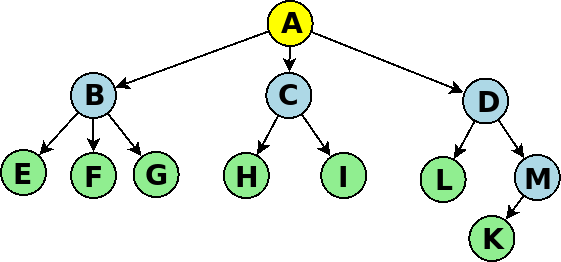
\includegraphics[width=0.7\linewidth]{img/tree_example}
	\label{fig:treeexample}
\end{figure}

Y para un mejor entendimiento asumiremos que los nodos hijos izquierdos serán todos menos el último hijo que será el derecho. De esta forma el nodo $B$ tiene dos hijos izquierdos ($E$,$F$) y un derecho ($G$).

\subsection{Recorrido en profundidad-primero}
\subsubsection{Preorden}

\emph{(\textbf{raíz}, izquierdo, derecho)}. Para recorrer un árbol no vacío en Preorden, hay que realizar
las siguientes operaciones recursivamente en cada nodo, comenzando con el nodo raíz:

\begin{itemize}
	\item Procesa la raíz
	\item Recorrer el subárbol izquierdo InOrden
	\item Recorrer el subárbol derecho InOrden
\end{itemize}

Si asumimos que el procesar la raiz es la impresión del valor almacenado en el nodo el recorrido en inorden en el árbol presentado de muestra anteriormente daría la siguiente secuencia o impresión de salida.

$$ A, B,E,F,G,C,H,I,D,L,M,K $$

\subsubsection{Inorden}

\emph{(izquierdo, \textbf{raíz}, derecho)}. El valor en un nodo no se procesa hasta que se procesen los valores en
su subárbol izquierdo.
Para recorrer un árbol no vacío en Inorden, hay que realizar las siguientes operaciones
recursivamente en cada nodo, comenzando con el nodo raíz:

\begin{itemize}
	\item Recorrer el subárbol izquierdo InOrden
	\item Procesa la raíz
	\item Recorrer el subárbol derecho InOrden
\end{itemize}

Si asumimos que el procesar la raiz es la impresión del valor almacenado en el nodo el recorrido en inorden en el árbol presentado de muestra anteriormente daría la siguiente secuencia o impresión de salida.

$$ E,F,B,G,H,C,I,A,L,D,K,M $$

\subsubsection{Postorden}

\emph{(izquierdo, derecho, \textbf{raíz})}. Para recorrer un árbol binario no vacío en Postorden, hay que realizar
las siguientes operaciones recursivamente en cada nodo, comenzando con el nodo raíz:

\begin{itemize}
	\item Recorrer el subárbol izquierdo InOrden
	\item Recorrer el subárbol derecho InOrden
	\item Procesa la raíz
\end{itemize}

Si asumimos que el procesar la raiz es la impresión del valor almacenado en el nodo el recorrido en inorden en el árbol presentado de muestra anteriormente daría la siguiente secuencia o impresión de salida.

$$ E,F,G,B,H,I,C,L,K,M,D,A $$

En general, la diferencia entre preorden, inorden y postorden es cuándo se recorre la raíz. En los tres, se recorre primero el sub-árbol izquierdo y luego el derecho. 

\begin{itemize}
	\item En preorden, la raíz se recorre antes que los recorridos de los subárboles izquierdo y derecho
	\item En inorden, la raíz se recorre entre los recorridos de los árboles izquierdo y derecho
	\item En postorden, la raíz se recorre después de los recorridos por el subárbol izquierdo y el derecho
\end{itemize}

Preorden (antes), inorden (en medio), postorden (después). 

\subsection{Recorrido en anchura-primero}
Los árboles también pueden ser recorridos en orden por nivel (de nivel en nivel), donde visitamos cada nodo en un nivel antes de ir a un nivel inferior. Esto también es llamado recorrido en anchura-primero o recorrido en anchura. Se etiquetan los nodos según su profundidad
(nivel). Se recorren ordenados de menor a mayor nivel, a igualdad de nivel
se recorren de izquierda a derecha.

Si asumimos que el procesar la raiz es la impresión del valor almacenado en el nodo el recorrido en anchura-primero en el árbol presentado de muestra anteriormente daría la siguiente secuencia o impresión de salida.

$$ A, B, C, D, E, F, G, H, I, L, M, K $$